\documentclass{article}

\usepackage{graphicx}
\usepackage{tikz}
\usepackage{tikzsymbols}
\usetikzlibrary{calc,patterns,shapes.geometric}
\pagestyle{empty}
\usepackage[margin=0pt]{geometry}
\geometry{papersize={14in,12in}}

\def\centerarc[#1](#2)(#3:#4:#5){\draw[#1] ($(#2)+({#5*cos(#3)},{#5*sin(#3)})$) arc (#3:#4:#5);}

\begin{document}
	\begin{figure}
		\centering
		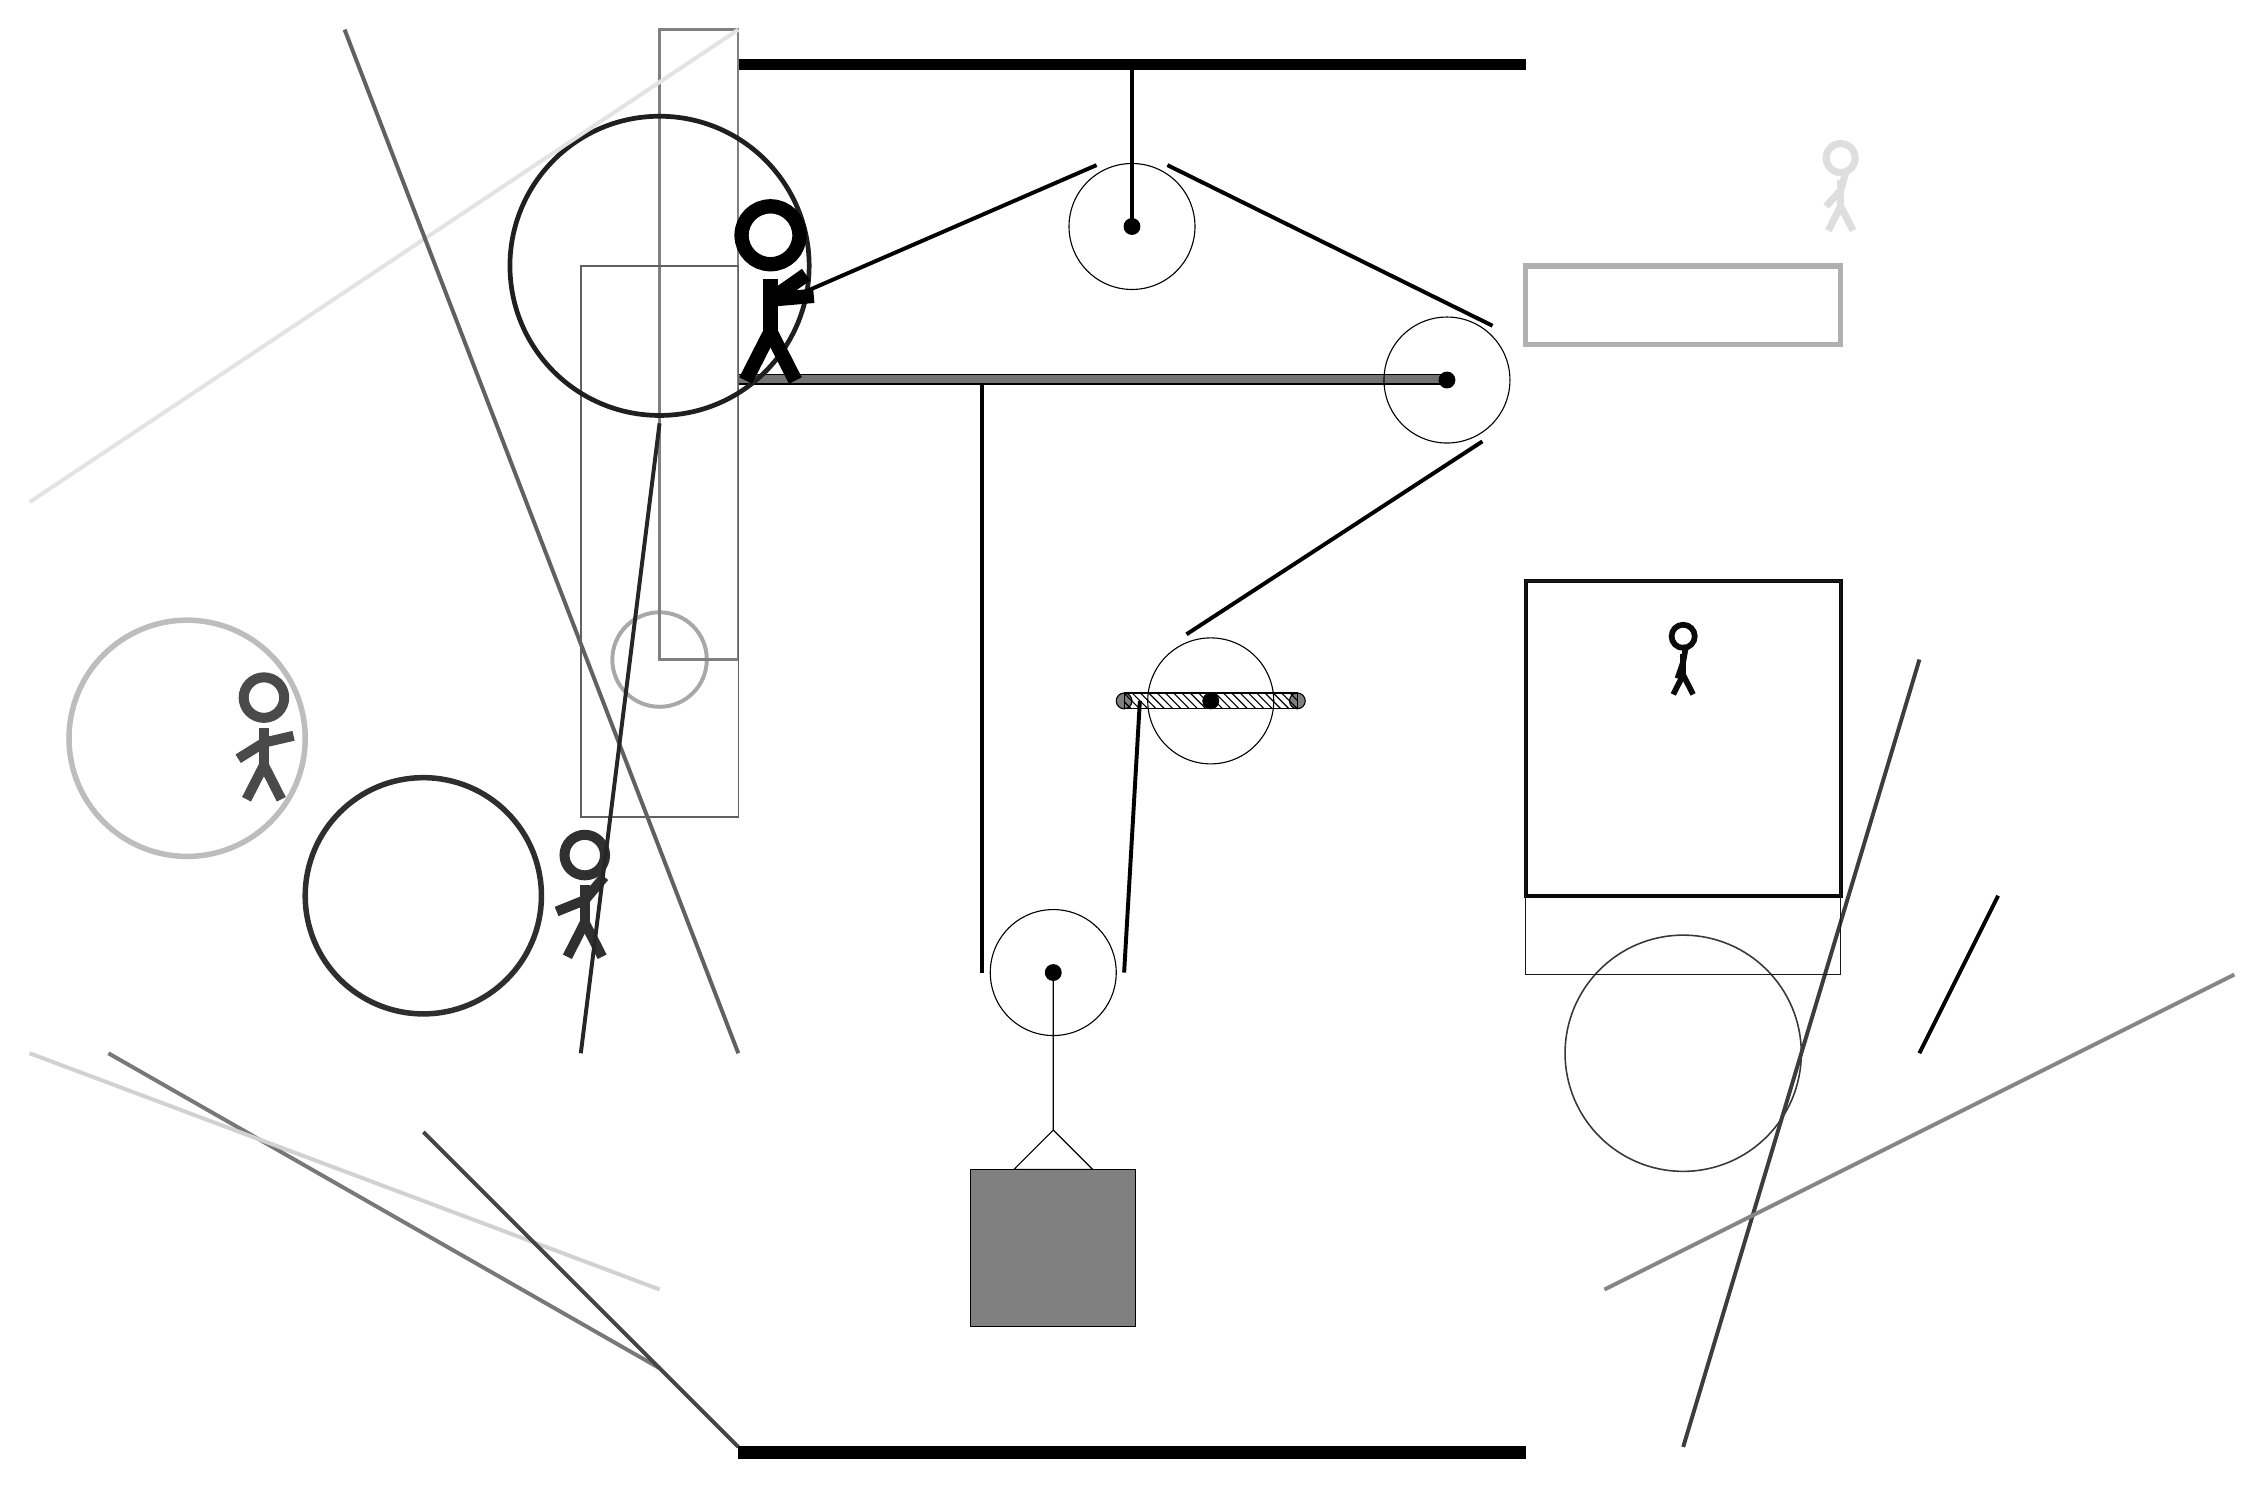
\begin{tikzpicture}
			%%%%% START %%%%%
			
			\draw[fill=black] (-2, 15.5) rectangle (8, 15.625);
			
			\draw[fill=black!55] (-2, 11.5) rectangle (7, 11.625);
			
			\draw (2, 4.025) circle (0.8);
			\draw[fill=black] (2, 4.025) circle (0.1);
			
			\node[line width=0.6mm, color=black!96] at (10, 8) {\Strichmaxerl[4][71][80]};
			
			\node[line width=0.5mm, color=black!81] at (-4, 5) {\Strichmaxerl[7][22][50]};
			\draw [line width=0.2mm, color=black!78](10, 3) circle (1.5);
			\draw[line width=0.5mm, color=black!96] (8, 5) rectangle (12, 9);
			
			\draw[line width=0.5mm, color=black!53](-3, -1) -- (-10, 3);
			\draw [line width=0.5mm, color=black!34](-3, 8) circle (0.6);
			
			\draw[line width=0.5mm, color=black!76](10, -2) -- (13, 8);
			\draw[line width=0.5mm, color=black!48](9, 0) -- (17, 4);
			\draw[line width=0.3mm, color=black!50] (-2, 16) rectangle (-3, 8);
			\draw[line width=0.2mm, color=black!62] (-4, 6) rectangle (-2, 13);
			\draw [line width=0.6mm, color=black!88](-3, 13) circle (1.9);
			\draw[line width=0.2mm, color=black!90] (8, 4) rectangle (12, 9);
			\draw[line width=0.5mm, color=black!18](-3, 0) -- (-11, 3);
			
			\draw [line width=0.7mm, color=black!82](-6, 5) circle (1.5);
			\draw[line width=0.5mm, color=black!11](-2, 16) -- (-11, 10);
			\draw [line width=0.7mm, color=black!26](-9, 7) circle (1.5);
			
			\draw[line width=0.5mm, color=black!98](13, 3) -- (14, 5);
			\draw[line width=0.5mm, color=black!62](-2, 3) -- (-7, 16);
			\draw[line width=0.5mm, color=black!73](-2, -2) -- (-6, 2);
			
			\draw[line width=0.5mm, color=black!85](-3, 11) -- (-4, 3);
			\node[line width=0.2mm, color=black!71] at (-8, 7) {\Strichmaxerl[7][32][13]};
			
			\node[line width=0.2mm, color=black!13] at (12, 14) {\Strichmaxerl[5][48][74]};
			
			\draw[line width=0.7mm, color=black!31] (8, 13) rectangle (12, 12);
			
			\draw (7, 11.55) circle (0.8);
			\draw[fill=black] (7, 11.55) circle (0.1);
			
			\draw[fill=white](4, 7.475) circle (0.8);
			\draw[fill=black] (4, 7.475) circle (0.1);
			\draw[fill=black!50] (2.9, 7.475) circle (0.1);
			\draw[fill=black!50] (5.1, 7.475) circle (0.1);
			\draw[pattern=north west lines, pattern color=black] (2.9, 7.575) rectangle (5.1, 7.375);
			
			\draw (3, 13.5) circle (0.8);
			\draw[fill=black] (3, 13.5) circle (0.1);
			\draw[line width=0.5mm] (3, 13.5) -- (3, 15.5);
			
			\draw (2, 4.025) -- (2, 2.025) -- (1.5, 1.525) -- (2.5, 1.525) -- (2, 2.025);
			\draw[fill=black!50] (0.95, 1.525) rectangle (3.05, -0.475);
			
			\draw[line width=0.5mm] (1.1, 11.5) -- (1.1, 4.025);
			\centerarc[line width=0.5mm](2, 4.025)(180:360:0.9);
			\draw[line width=0.5mm](2.9, 4.025) -- (3.1, 7.475);
			\centerarc[line width=0.5mm](4, 7.475)(110:180:0.9);
			\draw[line width=0.5mm](3.6922, 8.3207) -- (7.45, 10.7706);
			\centerarc[line width=0.5mm](7, 11.55)(-60:50:0.9);
			\draw[line width=0.5mm](7.5785, 12.2394) -- (3.45, 14.2794);
			\centerarc[line width=0.5mm](3, 13.5)(60:120:0.9);
			\draw[line width=0.5mm](2.55, 14.2794) -- (-1.2, 12.65);
			
			\node at (-1.5, 12.65) {\Strichmaxerl[10][-175][35]};
			
			\draw[fill=black] (-2, -2) rectangle (8, -2.15);
			
			%%%%% END %%%%%
		\end{tikzpicture}
	\end{figure}	
\end{document}